%%%%%%%%%%%%%%%%%%%%%%%%%%%%%%%%%%%%%%%%%%%%%%%%%%%%%%%%%%%%%%%%%%%%%%%
% 1. Document class
%%%%%%%%%%%%%%%%%%%%%%%%%%%%%%%%%%%%%%%%%%%%%%%%%%%%%%%%%%%%%%%%%%%%%%%

\documentclass[a4paper,12pt]{article}

%%%%%%%%%%%%%%%%%%%%%%%%%%%%%%%%%%%%%%%%%%%%%%%%%%%%%%%%%%%%%%%%%%%%%%%
% 2. Packages
%%%%%%%%%%%%%%%%%%%%%%%%%%%%%%%%%%%%%%%%%%%%%%%%%%%%%%%%%%%%%%%%%%%%%%%

% Tipo de input encoding
\usepackage[utf8]{inputenc}
\usepackage[spanish]{babel}

% Margen del documento
\usepackage[top = 2.5cm, bottom = 2.5cm, left = 2.5cm, right = 2.5cm]{geometry} 

% Para crear tablas
\usepackage{multirow}
\usepackage{booktabs}
\usepackage[table,xcdraw]{xcolor}

% Para manejo de gráficos y figuras
\usepackage{graphicx}
\usepackage{natbib}
\usepackage{float}

% Párrafos
\usepackage{setspace}
%\setlength{\parindent}{0cm}
%\setlength{\parskip}{1em}
%\renewcommand{\baselinestretch}{1.5}

% Cambiar el estilo de las listas
\renewcommand{\labelitemi}{$\bullet$}

% Para crear headers
\usepackage{fancyhdr}

% Para bibliografía
\usepackage{natbib}
\setcitestyle{numbers}

%%%%%%%%%%%%%%%%%%%%%%%%%%%%%%%%%%%%%%%%%%%%%%%%%%%%%%%%%%%%%%%%%%%%%%%
% 3. Header
%%%%%%%%%%%%%%%%%%%%%%%%%%%%%%%%%%%%%%%%%%%%%%%%%%%%%%%%%%%%%%%%%%%%%%%

% Crear el header
\pagestyle{fancy}
\fancyhf{}
\lhead{\footnotesize Reto III}
\rhead{\footnotesize Grupo 5}

% Colocar el número de la página
\cfoot{\footnotesize \thepage} 

%%%%%%%%%%%%%%%%%%%%%%%%%%%%%%%%%%%%%%%%%%%%%%%%%%%%%%%%%%%%%%%%%%%%%%%
% 4. Title
%%%%%%%%%%%%%%%%%%%%%%%%%%%%%%%%%%%%%%%%%%%%%%%%%%%%%%%%%%%%%%%%%%%%%%%

\begin{document}

\thispagestyle{empty}

% Header de la primera página
\begin{tabular}{p{14cm}}
{\large \bf Análisis Numérico} \\
Pontificia Universidad Javeriana \\ Semestre 2021-10 \\
\hline
% \\
\end{tabular}

% Título
\title{Reto III: Simulación de la Solución de \\ Sistemas de Ecuaciones Diferenciales}
\author{Alejandro Morales Contreras \\ Carlos Miguel Sánchez Loreto \\ Santiago Vásquez Sánchez}
\date{}

\begingroup
\let\newpage\relax
\maketitle
\endgroup

%%%%%%%%%%%%%%%%%%%%%%%%%%%%%%%%%%%%%%%%%%%%%%%%%%%%%%%%%%%%%%%%%%%%%%%
% 5. Body
%%%%%%%%%%%%%%%%%%%%%%%%%%%%%%%%%%%%%%%%%%%%%%%%%%%%%%%%%%%%%%%%%%%%%%%

\section{Introducción}

%\setlength{\parskip}{1em}

El presente documento pretende mostrar el análisis teórico, implementación y resultados obtenidos del reto III de la materia sobre la solución de sistemas de ecuaciones diferenciales mediante métodos numéricos, ahondando en el método de Euler y el método Runge-Kutta orden 4 para resolver EDO. Se simularon dos modelos asociados a los modelos epidemiológicos SI / SIR, y al modelo Depredador-Presa. \par

La implementación de los algoritmos fue llevada a cabo en el lenguaje de programación R, y los resultados fueron comparados mediante la herramienta Wolfram Alpha. Así mismo, se generaron dos Web Apps mediante la herramienta Shiny en R, para poder simular interactivamente ambos modelos mencionados.

%%%%%%%%%%%%%%%%%%%%%%%%%%%%%%%%%%%%%%%%%%%%%%%%%%%%%%%%%%%%%%%%%%%%%%%
% 5.1 Marco Teórico
%%%%%%%%%%%%%%%%%%%%%%%%%%%%%%%%%%%%%%%%%%%%%%%%%%%%%%%%%%%%%%%%%%%%%%%

\section{Marco Teórico}

\subsection{Métodos Numéricos para resolver Sistemas de EDO}

\subsubsection{Método de Euler}

El Método de Euler constituye el primer y más sencillo ejemplo de método numérico para la resolución de un problema de valor inicial de la forma:
 \[ y_0 = f(x, y) ,  y(x_0) = y_0 \]

Este método consiste en encontrar iterativamente la solución de una ecuación diferencial de primer orden y valores iniciales conocidos para un rango de valores. Partiendo de un valor inicial $x_0$ y avanzando con un paso $h$, se pueden obtener los valores de la solución de la siguiente manera:
\[ Y_{n+1} = Y_n + h · f(x_n, Y_n) \]
\[ x_n = x_{n-1} + h \]

Desde el punto de vista geométrico, tenemos en definitiva que el Método de Euler
aproxima a la función solución por medio de una línea poligonal, la aproximación será menos precisa cuanto mayor sea en número de pasos, es decir, cuanto más “lejos” nos encontremos del punto inicial $(x_0, y_0)$. Por otro lado, el error será evidentemente mayor cuanto más grande sea el “paso” del método, h.

\subsubsection{Método Runge-Kutta}

Uno de los métodos más utilizados para resolver numéricamente problemas de ecuaciones diferenciales ordinarias con condiciones iniciales es el método de Runge-Kutta de cuarto orden, el cual proporciona un pequeño margen de error con respecto a la solución real del problema y es fácilmente programable en un software como R para realizar las iteraciones necesarias. \par

Es profundamente conveniente para casos en los que la solución no puede hallarse por los métodos convencionales (como separación de variables). Hay variaciones en el
método de Runge-Kutta de cuarto orden pero el más utilizado es el método en el
cual se elige un tamaño de paso $h$ y un número máximo de iteraciones $n$ tal que: \par

\begin{itemize}
    \item $k_1 = f(x_n,t_n)$.
    \item $k_2 = f(x_n +\frac{h}{2}k_1 , t_n + \frac{h}{2} )$   
    \item $k_3 = f(x_n + \frac{h}{2}k_2 , t_n + \frac{h}{2})$ 
    \item $k_4 = f(x_n + hk_3 , t_n+ h)$
\end{itemize}

Dados los valores $k_i$ anteriores se puede modelar la ecuación para cada iteración de la siguiente manera: \par

\[y_{n+1} = y_n + \frac{1}{6}[k_1 + 2k_2 + 2k_3 + k_4]  \]
 
\subsection{Modelos Epidemiológicos}

\subsubsection{Modelo SI}

El modelo $"SI"$ es el más simple posible. La población está formada sólo por
Susceptibles(S) e Infectados(I), y si se contagia un individuo, la enfermedad es permanente, es decir, no existe la posibilidad de recuperación. \par

Consiste en un sistema de dos ecuaciones diferenciales en el que aparecen el número
$S(t)$ de personas susceptibles y el número $I(t)$ personas infectadas como variables dependientes del tiempo $t$ De acuerdo con la ley de acción de masas, la razón de cambio de susceptible a infectado es proporcional al producto del tamaño de ambas poblaciones:

El sistema de ecuaciones que representa el Modelo epidemiológico SI es la siguiente:

\begin{eqnarray}
   \frac{dS}{dt} = -ßSI \\
    \nonumber \\
   \frac{dI}{dt} = +ßSI  
\end{eqnarray}


\subsubsection{Modelo SIR}
El modelo SIR es un modelo epidemiológico capaz de capturar muchas de las características típicas de los brotes epidérmicos. El nombre del modelo proviene de las iniciales $S$(población $S$uceptible), $I$(población $I$nfectada) y $R$(población $R$ecuperada). \par

Este modelo relaciona las variaciones de las tres poblaciones ($S$, $I$, $R$) a través de la tasa de infección y por medio del período de infección promedio. La población total es $N = S+I+R$, planteada esta partición de la población total, se requieren ecuaciones que especifiquen y describan la variacion temporal del número de individuos en cada compartimiento. El numero de individuos en cada compartimiento deben ser números enteros, aunque dado el tamaño de la población N, las particiones $S, I, R$ pueden ser tratadas como variables continuas.\par

El modelo $SIR$ viene dado por el siguiente sistema de ecuaciones diferenciales:\par

\[ \frac{dS}{dt} = -\beta SI \]

\vspace{-1em}

\[ \frac{dI}{dt} = + \beta SI - \gamma I \]

\vspace{-1em}

\[ \frac{dR}{dt} = \gamma I \]

En el sistema de ecuaciones, la tasa de transmisión esta representada por la letra griega $\beta$ y la tasa de recuperación por la letra $\gamma$. \par

\subsection{Modelo Depredador-Presa}

 El modelo de ecuaciones de Lotka-Volterra, también conocido como modelo Depredador-Presa, es un modelo conformado por dos ecuaciones diferenciales de primer orden no lineales que se usan para describir dinámicas de sistemas biológicos en los que dos especias interactúan, una como depredador y una como presa. Este par de ecuaciones fueron creadas e implementadas inicialmente y de forma independiente por Alfred J. Lotka en 1925 y Vito Volterra en 1926 (de ahí su nombre).\par
 
 El sistema de ecuaciones se define como: \par

\[ \frac{dx}{dt}  = x(\alpha - \beta y) \]

\vspace{-1em}

\[ \frac{dy}{dt} = -y(\gamma -\delta x) \]

Donde: \par

\begin{itemize}
    \item x es la cantidad de presas
    \item y es la cantidad de depredadores
    \item $\frac{dy}{dt}$ y $\frac{dx}{dt}$ representan el crecimiento de las dos poblaciones en el tiempo
    \item t representa el tiempo
    \item $\alpha$ es la tasa de crecimiento de las presas
    \item $\beta$ es el éxito en la caza del depredador
    \item $\gamma$ es la tasa de decrecimiento de los depredadores
    \item $\delta$ es el éxito en la caza y cuánto alimenta cazar una presa al depredador
\end{itemize}
 
%%%%%%%%%%%%%%%%%%%%%%%%%%%%%%%%%%%%%%%%%%%%%%%%%%%%%%%%%%%%%%%%%%%%%%%
% 5.2 Problema Planteado
%%%%%%%%%%%%%%%%%%%%%%%%%%%%%%%%%%%%%%%%%%%%%%%%%%%%%%%%%%%%%%%%%%%%%%%

\section{Problema Planteado}

\subsection{Simulación del Covid-19 mediante los modelos SI / SIR}

A partir de la base de datos tomada de la European Centre for Disease Prevention and Control (ECDC) se plantea utilizar la información de una fecha y un país seleccionado para la configuración de los modelos SI y SIR, con el fin de analizar el comportamiento del virus COVID-19 en un tiempo $t$.   \par

\subsection{Simulación del modelo Depredador-Presa}

Utilizando como datos reales, el índice de capturas de linces y conejos elaborada por la compañía Hudson Bay entre los años 1900 y 1920, se busca modelar el comportamiento Depredador-Presa utilizando métodos númericos como Euler y Runge-Kutta para el estudio del cremiento exponencial de la población de animales, así como también el análisis de las tasas de natalidad y mortalidad en un tiempo $t$ determinado. \par
Adicionalmente se realizan pruebas del comportamiento del modelo para valores arbitrarios con la finalidad de comparar ambas situaciones planteadas.

%%%%%%%%%%%%%%%%%%%%%%%%%%%%%%%%%%%%%%%%%%%%%%%%%%%%%%%%%%%%%%%%%%%%%%%
% 5.3 Resultados Obtenidos
%%%%%%%%%%%%%%%%%%%%%%%%%%%%%%%%%%%%%%%%%%%%%%%%%%%%%%%%%%%%%%%%%%%%%%%

\section{Resultados Obtenidos}

\subsection{Simulación del Covid-19 mediante los modelos SI / SIR}

A continuación se presentan los resultados obtenidos, al simular el virus del Covid-19 en Colombia, empezando el día 20 de abril del 2020, con 300 días de tiempo de simulación.

\subsubsection{Modelo SI}

En la figura \ref{fig:si_euler} se presentan los resultados obtenidos de la simulación mediante el modelo SI con el método de Euler.

\begin{figure}[ht!]
\centering
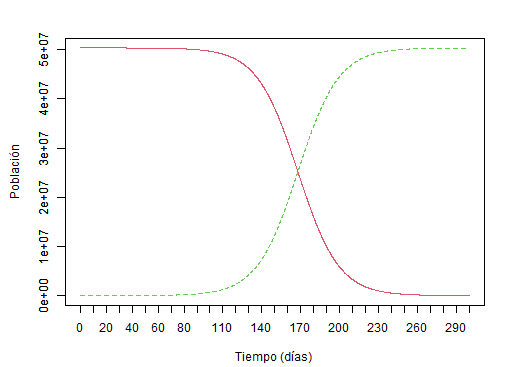
\includegraphics[scale=0.7]{img/ModeloEpedemiologico_SI_Euler.PNG}
\vspace{-1em}
\caption{Modelo Epidemiológico SI por el método de Euler}
\label{fig:si_euler}
\end{figure}  \par

\newpage

Al hacer un análisis sobre los datos, se puede ver como en Colombia, casi la totalidad de la población se encontraba en estado susceptible, y solo unas pocas personas se encontraban infectadas en el día 0. Conforme fue avanzando el tiempo, la cantidad de personas infectadas comenzó a elevarse, mientras que la cantidad de personas susceptibles empezó a bajar, hasta que la totalidad de la población se encontraba infectada después de 290 días. \par

Como es común de los modelos SI, eventualmente toda la población se encontrará infectada, dada una velocidad de infección positiva. \par

En la figura \ref{fig:si_rk4} se presentan los resultados obtenidos de la simulación mediante el modelo SI con el método de Runge-Kutta orden 4.

\begin{figure}[ht!]
\centering
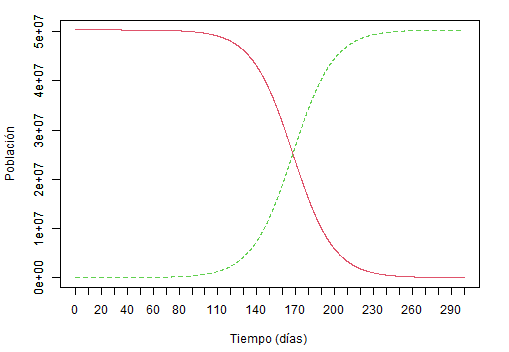
\includegraphics[scale=0.7]{img/ModeloEpedemiologico_SI_RungeKutta.PNG}
\vspace{-1em}
\caption{Modelo Epidemiológico SI por el método de Runge-Kutta}
\label{fig:si_rk4}
\end{figure}  \par

Tal como la simulación siguiendo el método de Euler, la totalidad de la población se encuentra infectada al cabo de aprox. 290 días. Así mismo, las curvas siguen unas trayectorias muy similares. \par

\subsubsection{Modelo SIR}

En la figura \ref{fig:sir_euler} se presentan los resultados obtenidos de la simulación mediante el modelo SIR con el método de Euler.

\begin{figure}[ht!]
\centering
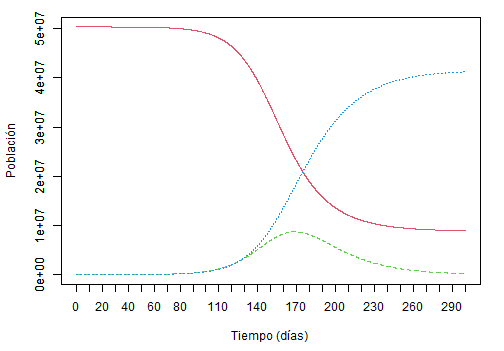
\includegraphics[scale=0.7]{img/ModeloEpedemiologico_SIR_Euler.PNG}
\vspace{-1em}
\caption{Modelo Epidemiológico SIR por el método de Runge-Kutta}
\label{fig:sir_euler}
\end{figure}  \par

\newpage 

Analizando los resultados, encontramos grandes diferencias en el comportamiento con el modelo SI. Al cabo de los 300 días, la totalidad de la población susceptible no sigue siendo 0, sino que no se ha logrado infectar a toda la población. La cantidad de personas infectadas tampoco es acumulativa, sino que las personas son retiradas apenas culmina el periodo infeccioso, y pasan a ser la curva azul ilustrada. Ocurre un pico de la pandemia a los 170 días de la simulación, y después se aplana la curva, empezando a crecer la cantidad de personas retiradas. \par

En la figura \ref{fig:sir_rk4} se presentan los resultados obtenidos de la simulación mediante el modelo SIR con el método de Runge-Kutta orden 4.

\begin{figure}[ht!]
\centering
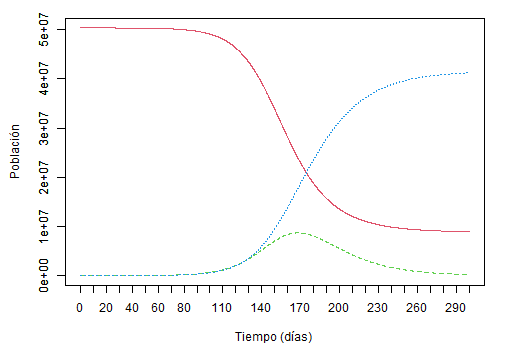
\includegraphics[scale=0.7]{img/ModeloEpedemiologico_SIR_RungeKutta.PNG}
\vspace{-1em}
\caption{Modelo Epidemiológico SIR por el método de Runge-Kutta}
\label{fig:sir_rk4}
\end{figure}  \par

Tal como los resultados obtenidos mediante el método de Euler, no se logra infectar a toda la población susceptible, ocurre un pico de la pandemia al día 170, y se logra aplanar la curva de infección. \par

\subsection{Simulación del modelo Depredador-Presa}

A continuación se presentan los resultos obtenidos al simular el modelo Depredador-Presa utilizando los siguientes datos sobre las especies Conejos y Linces capturadas por la compañía Hudson Bay en Canadá, entre los años 1900 y 1920:

\begin{itemize}
    \item Presas iniciales = $30$.
    \item Depredadores iniciales = $4$  
    \item Tasa de crecimiento de las presas = $0.4$
    \item Tasa de éxito en la caza del depredador = $0.018$
    \item Tasa de decrecimiento de los depredadores = $0.8$
    \item Tasa de alimento por cada presa que consume el depredador = $0.023$
\end{itemize}

En la figura \ref{fig:dp_euler} se presentados los resultados de la simulación mediante el modelo DP de Lotka-Voltera con el método de Euler y tamaño del paso $0.1$.

\begin{figure}[ht!]
\centering
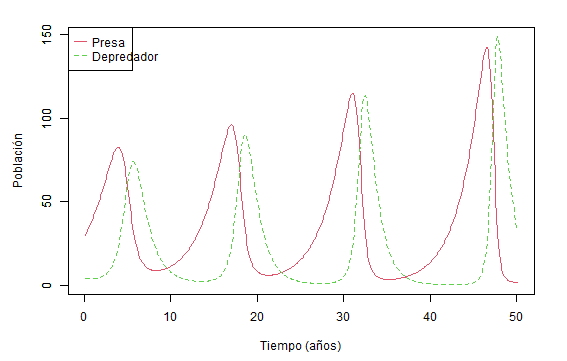
\includegraphics[scale=0.7]{img/DepredadorPresa_Euler.PNG}
\vspace{-1em}
\caption{Modelo Depredador-Presa por el método de Euler}
\label{fig:dp_euler}
\end{figure} 
\newpage

Analizando los resultados, podemos ver como la cantidad de presas y depredadores siguen curvas similares, cada vez alcanzando picos más altos entre las poblaciones de presas y depredadores. El comportamiento indica que las presas pueden crecer rápidamente en ausencia de depredadores, pero cuando estas empiezan a aumentar bastante, la cantidad de depredadores también (debido a más alimento disponible). Finalmente, ambas poblaciones se reducen y vuelve a empezar el ciclo.

En la figura \ref{fig:dp_rk4} se presentan los resultados obtenidos de la simulación mediante el modelo DP de  Lotka-Voltera  con el método de Runge-Kutta orden 4 y tamaño del paso $0.1$.

\begin{figure}[ht!]
\centering
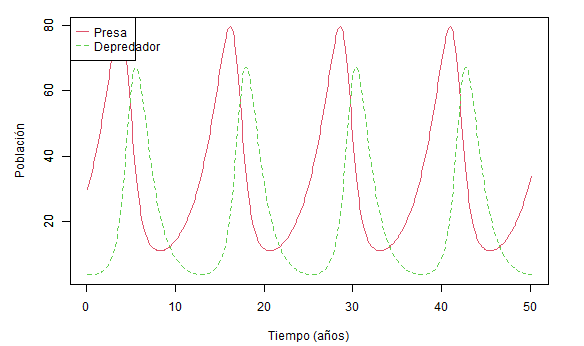
\includegraphics[scale=0.7]{img/DepredadorPresa_RungeKutta.PNG}
\vspace{-1em}
\caption{Modelo Depredador-Presa por el método de Runge-Kutta orden 4}
\label{fig:dp_rk4}
\end{figure} \par

Analizando los resultados, podemos encontrar notables diferencias con la simulación mediante el método de Euler. Los picos alcanzados por ambas poblaciones son más pequeños, y no empiezan a crecer cada vez más alto conforme al tiempo. Así mismo, la cantidad de depredadores nunca sobrepasa la de presas, y siguen un ciclo casi periódico en su relación. \par

\newpage

%%%%%%%%%%%%%%%%%%%%%%%%%%%%%%%%%%%%%%%%%%%%%%%%%%%%%%%%%%%%%%%%%%%%%%%
% 5.4 Web Apps
%%%%%%%%%%%%%%%%%%%%%%%%%%%%%%%%%%%%%%%%%%%%%%%%%%%%%%%%%%%%%%%%%%%%%%%

\section{Web Apps}

Con el fin de generar herramientas de visualización más amigables, que permitieran probar varios conjuntos de datos en tiempo real y de manera interactiva, se crearon dos Web Apps en el lenguaje de programación R, con ayuda de la librería Shiny. Las aplicaciones creadas son totalmente funcionales, y se pueden encontrar en el siguiente repositorio: \par

https://github.com/amoralesc/analisis-numerico.git \par

\subsection{Simulación del Covid-19 mediante los modelos SI / SIR}

La Web App permite la simulación del virus Covid-19 en un país, en una fecha y rango de tiempo especificados. En la figura \ref{fig:demo1_entrada} se muestra como luce la entrada de datos. Los datos se cargan directamente desde la base de datos prestada por el ECDC.

\begin{figure}[ht!]
\centering
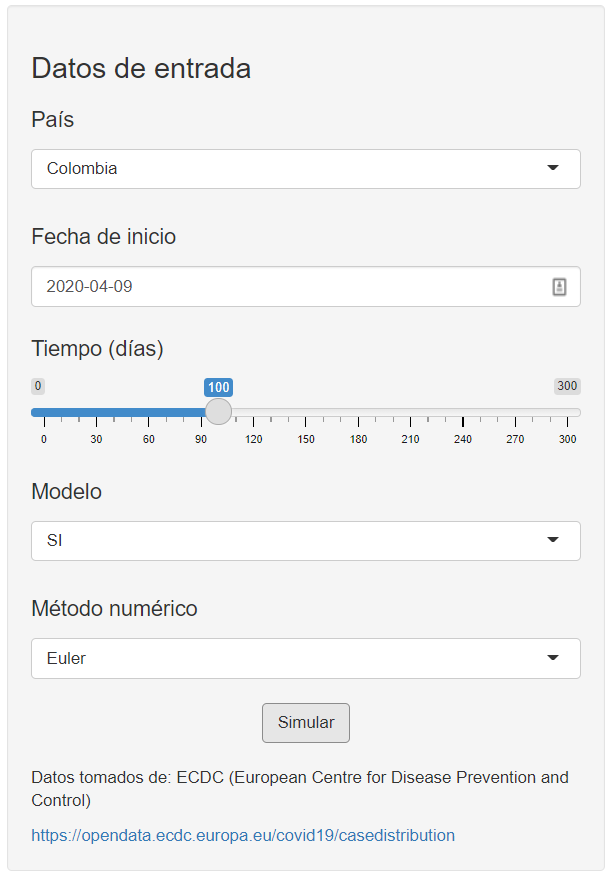
\includegraphics[scale=0.4]{img/demo1_entrada}
\vspace{-1em}
\caption{Datos de entrada de la Web App Simulación del Covid-19}
\label{fig:demo1_entrada}
\end{figure} \par

Como podemos ver, se debe escoger el país a simular, la fecha de inicio, el rango de tiempo en días, el modelo (SI o SIR) y el método numérico a utilizar (Euler o Runge-Kutta orden 4). La salida de la Web App es la gráfica de la simulación del virus en el tiempo, como se muestra en la figura \ref{fig:demo1_salida}.

\begin{figure}[ht!]
\centering
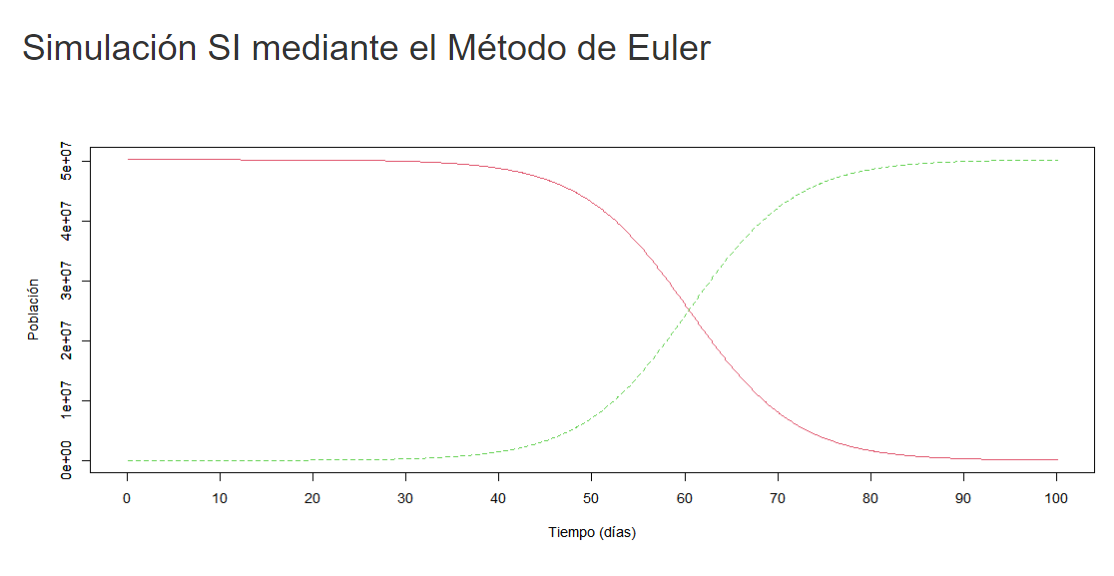
\includegraphics[scale=0.4]{img/demo1_salida}
\vspace{-1em}
\caption{Salida de la Web App Simulación del Covid-19}
\label{fig:demo1_salida}
\end{figure} \par

\subsection{Simulación del modelo Depredador-Presa}

La Web App permite la simulación del modelo Depredador-Presa de Lotka-Volterra, para dos especies calculadas. En la figura \ref{fig:demo2_entrada} se muestra como luce la entrada de datos. Los datos se cargan de un ejemplo, o por variables propias.

\begin{figure}[ht!]
\centering
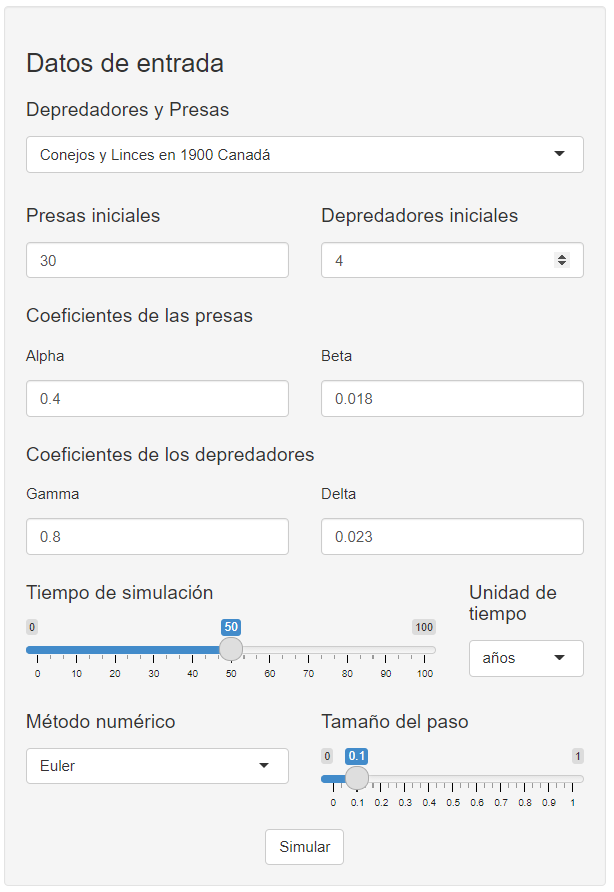
\includegraphics[scale=0.45]{img/demo2_entrada}
\vspace{-1em}
\caption{Datos de entrada de la Web App Simulación Depredador-Presa}
\label{fig:demo2_entrada}
\end{figure} \par

Como podemos ver, se debe escoger las especies a simular, las cantidades de presas y depredadores iniciales, los coeficientes alpha, betta, gamma y delta, el tiempo de la simulación, el método numérico a utilizar (Euler o Runge-Kutta orden 4) y el tamaño del paso. La salida de la Web App es la gráfica de las poblaciones de las especies en el tiempo, como se muestra en la figura \ref{fig:demo2_salida}.

\begin{figure}[ht!]
\centering
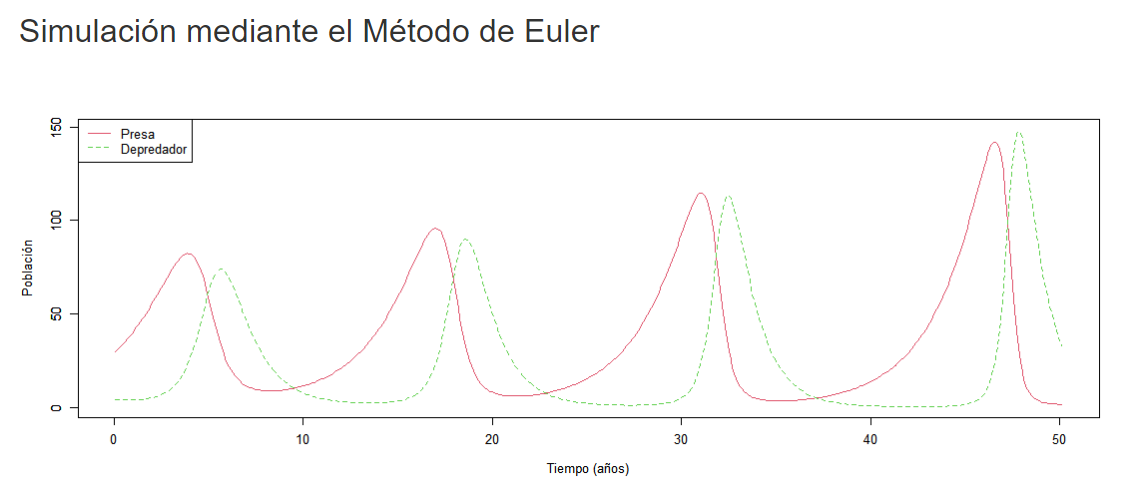
\includegraphics[scale=0.5]{img/demo2_salida}
\vspace{-1em}
\caption{Salida de la Web App Simulación Depredador-Presa}
\label{fig:demo2_salida}
\end{figure} \par

\newpage

%%%%%%%%%%%%%%%%%%%%%%%%%%%%%%%%%%%%%%%%%%%%%%%%%%%%%%%%%%%%%%%%%%%%%%%
% 5.5 Conclusiones
%%%%%%%%%%%%%%%%%%%%%%%%%%%%%%%%%%%%%%%%%%%%%%%%%%%%%%%%%%%%%%%%%%%%%%%

\section{Conclusiones}

Después de realizar toda la investigación e implementación de los algoritmos utilizando librerías internas y externas para calcular las soluciones a sistemas de ecuaciones diferenciales, así como la graficación de sus resultados en función del tiempo, podemos resaltar la importancia de la utilización de estos métodos para resolver dichos sistemas. Un sistema de ecuaciones diferencial, suele describir aspectos o situaciones de la vida real, muchas veces en función del tiempo. Con dos ejemplos de la vida real, evidenciamos como podemos modelar tanto la propagación de un virus, como la convivencia entre dos especies. \par

Por otra parte, los métodos númericos de Euler y Runge-Kutta orden 4, son muy útiles a la hora de resolver ecuaciones diferenciales no lineales. También aquellas que no pueden ser resueltas de manera análitica. Ya que se resuelven iterativamente, es posible calcular datos que con los métodos tradicionales no sería posible. \par

Mediante el desarrollo de los Web App Simulación del Covid-19 y Simulación Depredador-Presa por medio del paquete componente Shiny R de Rstudio, realizamos un aprendizaje directo del desarrollo de Web Apps y de como hacerlo en la herramienta RStudio. También se logró entender e implementar de manera correcta tanto los modelos epidemiológicos SI, SIR y el modelo Depredador-Presa, y tuvimos la capacidad de poder variar los datos interactivamente. \par

Sobre los modelos epidemiológicos simulados, podemos decir que estos buscan simular la propagación de algún tipo de infección, pero que sus parámetros de entrada pueden llegar a ser muy variables y pueden variar la solución presentada. Para el modelo SI, la conclusión siempre será que todos los individuos del sistema terminarán infectados, siempre que la propagación $\beta$ sea positiva. Sin embargo, esto no ocurre así en la vida real, ya que personas que son infectadas y pasan por el periodo de infección, casi nunca vuelven a estar infectadas, y alivianan la cantidad de personas susceptibles que se enferman. Es por esto que concluímos que el modelo SIR es mucho más útil para aproximar una situación de la propagación de una infección. \par

Sobre el modelo Depredador-Presa de Lotka-Volterra, pudimos realizar distintas simulaciones variando los parámetros de las especies. En general, aunque se necesita un conjunto de condiciones preliminares para aceptar este modelo como uno que refleje lo que pasa en la naturaleza, sigue siendo una buena forma de representar como interactuarían dos especies de presas y depredadores en un ambiente aíslado. \par

\newpage

%%%%%%%%%%%%%%%%%%%%%%%%%%%%%%%%%%%%%%%%%%%%%%%%%%%%%%%%%%%%%%%%%%%%%%%
% 6 Referencias
%%%%%%%%%%%%%%%%%%%%%%%%%%%%%%%%%%%%%%%%%%%%%%%%%%%%%%%%%%%%%%%%%%%%%%%

\bibliographystyle{IEEEtranN}
\bibliography{References}

\begin{thebibliography}{00}
\bibitem{b1} R. L. Burden y J. D. Faires, Numerical analysis, 9th ed. Boston, MA: Brooks/Cole, Cengage Learning, 2011.

\bibitem{b2} Métodos Numéricos en Ecuaciones Diferenciales Ordinarias (Tema 4) [Online]. Available: https://campus.usal.es/~mpg/Personales/PersonalMAGL/Docencia/MetNum

Tema4Teo(09-10).pdf

\bibitem{b3} Método de Runge-Kutta para Ecuaciones Diferenciales.[Online]. Available: https://repositorio.upct.es/bitstream/handle/10317/282/ANEXO\%\$20V.M\%\$C3\%
89TODO\%20DE\%20RUNGE-KUTTA..pdf?sequence=8\&isAllowed=y

\bibitem{b4} J.H. Wilches \& M. C. Castillo, Aproximación matemática del modelo epidemiologíco SIR para la comprensión de las medidas de contención contra el Covid-19, Revista Española de Salud Pública, vol. 94, no. 11, 23 de septiembre de 2020.

\bibitem{b5} L. García Rovira, Modelos Matemáticos Compartimentales en Epidemiología, Universidad de La Laguna, pp. 14-22,2020.

\bibitem{b6} A. Sáez (2015/01/05), Ecuaciones de Lotka-Volterra: modelo presa depredador [Online], Avalilable: https://pybonacci.org/2015/01/05/ecuaciones-de-lotka-volterra-modelo-presa-depredador/

\bibitem{b7} Modelo Lotka-Volterra (Práctica 5). [Online]. Available: http://matema.ujaen.es/jnavas/web\_modelos/labiologia/practica5.pdf
\end{thebibliography}
\end{document}

%%%%%%%%%%%%%%%%%%%%%%%%%%%%%%%%%%%%%%%%%%%%%%%%%%%%%%%%%%%%%%%%%%%%%
% Ejemplos
%%%%%%%%%%%%%%%%%%%%%%%%%%%%%%%%%%%%%%%%%%%%%%%%%%%%%%%%%%%%%%%%%%%%%

%%%%%%%%%%%%%%%%%%%%%%% Insertar Imágenes %%%%%%%%%%%%%%%%%%%%%%%%%%
%\begin{figure}[h!]
%\centering
%\includegraphics[scale=1.7]{img/ruta.jpg}
%\caption{Nombre de la figura}
%\label{fig:etiqueta}
%\end{figure}
